\documentclass[11pt,a4paper]{article}
\usepackage[margin=23mm]{geometry}
\usepackage{amsmath,amssymb,amsthm,mathtools,booktabs,microtype}
\usepackage[colorlinks=true,linkcolor=blue!40!black,urlcolor=blue!40!black,citecolor=blue!40!black]{hyperref}
\usepackage{xcolor,fancyhdr,graphicx}
\pagestyle{fancy}\fancyhf{}\fancyhead[L]{Trotter error estimation for HHL}\fancyfoot[C]{\thepage}
\setlength{\headheight}{14pt}\setlength{\parindent}{0pt}\setlength{\parskip}{4pt}
\newcommand{\norm}[1]{\left\lVert #1\right\rVert}
\newcommand{\ii}{\mathrm{i}}
\newcommand{\CC}{C_{\mathrm{comm}}}
\newtheorem{theorem}{Theorem}
\title{Trotter Error Estimation for HHL\\[4pt]\large Unitary error, effective-matrix error, and step selection}
\author{HHL paper revision --- standalone derivation}
\date{9 September 2026}
\begin{document}
\maketitle
\begin{abstract}
For a Hermitian decomposition $H=\sum_a H_a$, first-order Trotterization with $r$ steps over evolution time $\tau$ has operator error at most $\tau^2\CC/(2r)$, where $\CC=\sum_{a<b}\norm{[H_a,H_b]}$. If the microstep $h=\tau/r$ satisfies $h\sum_a\norm{H_a}\leq1/2$, a convergent matrix-logarithm argument also gives a Hermitian effective matrix with error at most $h\CC$. This note proves both bounds and explains the shared-microstep condition needed to use the second bound in HHL. A numerical study of 850 matrices (20,400 paired measurements) compares actual spectral-norm errors with both bounds, including step-size, dimension and branch-condition sweeps. The estimates are deterministic and do not extrapolate numerical histograms.
\end{abstract}

\section{Setup and the two different errors}
Let $H_1,\ldots,H_L\in\mathbb C^{N\times N}$ be Hermitian, with
\begin{equation}
 H=\sum_{a=1}^L H_a,\qquad
 B=\sum_{a=1}^L\norm{H_a},\qquad
 \CC=\sum_{1\leq a<b\leq L}\norm{[H_a,H_b]}.
\end{equation}
Here $[A,B]=AB-BA$, and all matrix norms are spectral norms. No restriction on nonzero positions is needed; the result applies in particular to one-sparse decompositions used in HHL.

Define one ordered microstep and the repeated formula by
\begin{equation}
 P(h)=e^{\ii H_1h}\cdots e^{\ii H_Lh},\qquad
 S_r(\tau)=P(\tau/r)^r,\qquad r\in\mathbb N_{\geq1}.
\end{equation}
Two quantities must be distinguished:
\begin{align}
 E_U&=\norm{S_r(\tau)-e^{\ii H\tau}}
 &&\text{(unitary or operator error)},\\
 E_H&=\norm{\widehat H-H}
 &&\text{(effective-matrix error)}.
\end{align}
$E_U$ is dimensionless. $E_H$ has the units of $H$; evolution time has inverse units of $H$. All quantities can be taken dimensionless after a declared matrix normalization. The second error requires a justified definition of $\widehat H$, not merely a small value of $E_U$.

\section{The unitary-error bound}
\begin{theorem}[First-order Trotter error]\label{thm:unitary}
For every finite Hermitian decomposition, every real $\tau$, and every integer $r\geq1$,
\begin{equation}\label{eq:unitary}
 \boxed{\norm{S_r(\tau)-e^{\ii H\tau}}
 \leq\min\left\{2,\frac{\tau^2\CC}{2r}\right\}.}
\end{equation}
\end{theorem}

\subsection{One step with two terms}
For two Hermitian matrices $A,D$, set
\begin{equation}
 V(t)=e^{\ii At}e^{\ii Dt},\qquad U(t)=e^{\ii(A+D)t}.
\end{equation}
Direct differentiation gives the exact differential equation
\begin{align}
 V'(t)&=\ii(A+D)V(t)+R(t),\\
 R(t)&=\left(e^{\ii At}\ii D e^{-\ii At}-\ii D\right)V(t).
\end{align}
The conjugation difference is an integral of a commutator:
\begin{equation}
 e^{\ii At}\ii D e^{-\ii At}-\ii D
 =\int_0^t e^{\ii Av}[\ii A,\ii D]e^{-\ii Av}\,dv.
\end{equation}
For $t\geq0$, unitary invariance of the spectral norm gives
\begin{equation}
 \norm{R(t)}\leq t\norm{[A,D]}.
\end{equation}
Variation of parameters then yields
\begin{align}
 V(t)-U(t)&=\int_0^t U(t-u)R(u)\,du,\\
 \norm{V(t)-U(t)}&\leq\int_0^t u\norm{[A,D]}\,du
 =\frac{t^2}{2}\norm{[A,D]}.
\end{align}
The factor $t^2/2$ is the area of the double-integral region. The proof is exact; no higher-order Taylor or Dyson terms have been discarded. Negative times follow by replacing $A,D$ with $-A,-D$.

\subsection{One step with many terms}
Successively split the first remaining term from the sum of all later terms. At split $a$, the two-term bound contributes at most
\begin{equation}
 \frac{h^2}{2}\norm{\left[H_a,\sum_{b>a}H_b\right]}
 \leq\frac{h^2}{2}\sum_{b>a}\norm{[H_a,H_b]}.
\end{equation}
Telescoping the splits, with all surrounding factors unitary, gives
\begin{equation}\label{eq:local}
 \norm{P(h)-e^{\ii Hh}}\leq\frac{h^2}{2}\CC.
\end{equation}
The grouped-commutator version is Proposition 15 of Childs et al.~\cite{childs}; the pairwise sum used here follows by the triangle inequality.

\subsection{Accumulation over repeated steps}
For any unitaries $V,W$,
\begin{equation}
 V^r-W^r=\sum_{k=0}^{r-1}V^{r-1-k}(V-W)W^k,
 \qquad \norm{V^r-W^r}\leq r\norm{V-W}.
\end{equation}
Taking $V=P(h)$, $W=e^{\ii Hh}$ and $h=\tau/r$ gives
\begin{equation}
 E_U\leq r\frac{h^2\CC}{2}=\frac{\tau^2\CC}{2r}.
\end{equation}
The independent ceiling two follows from the triangle inequality for two unitary matrices. This proves Theorem~\ref{thm:unitary}.

\section{A rigorous effective-matrix bound}
A small unitary error at one time does not alone imply a small matrix error: unitary eigenphases are defined modulo $2\pi$, and logarithms have branches. The following sufficient step-size condition fixes the branch explicitly.

\begin{theorem}[Effective matrix of a microstep]\label{thm:matrix}
Suppose $h>0$ and $hB\leq1/2$. Then
\begin{equation}
 \widehat H=\frac{\operatorname{Log}P(h)}{\ii h}
\end{equation}
is Hermitian, $P(h)=e^{\ii\widehat Hh}$, and
\begin{equation}\label{eq:matrix}
 \boxed{\norm{\widehat H-H}
 \leq\frac{h\CC}{2(1-hB)}\leq h\CC.}
\end{equation}
Here $\operatorname{Log}$ is the principal matrix logarithm.
\end{theorem}

\subsection{Step-size control of the logarithm branch}
Since $H_a$ is Hermitian,
\begin{equation}
 e^{\ii H_ah}-I=\int_0^h\ii H_a e^{\ii H_au}\,du,
 \qquad\norm{e^{\ii H_ah}-I}\leq h\norm{H_a}.
\end{equation}
Telescoping the product around identity therefore gives
\begin{equation}\label{eq:nearidentity}
 \norm{P(h)-I}\leq hB,\qquad
 \norm{e^{\ii Hh}-I}\leq h\norm H\leq hB.
\end{equation}
Consequently both matrices lie in the norm ball of radius $1/2$ around identity. The logarithm series converges there. Because $P(h)$ is unitary, its principal logarithm is skew-Hermitian, so $\widehat H$ is Hermitian. Also $h\norm H\leq1/2<\pi$, and hence
\begin{equation}
 \operatorname{Log}(e^{\ii Hh})=\ii Hh.
\end{equation}

\subsection{A logarithm difference inequality}
For matrices $X,Y$ with $\norm X,\norm Y\leq\rho<1$,
\begin{equation}
 \log(I+X)=\sum_{k=1}^{\infty}\frac{(-1)^{k+1}}{k}X^k.
\end{equation}
No commutativity between $X$ and $Y$ is required: telescoping gives
\begin{equation}
 \norm{X^k-Y^k}\leq k\rho^{k-1}\norm{X-Y}.
\end{equation}
Absolute convergence then permits the bound
\begin{align}
 \norm{\log(I+X)-\log(I+Y)}
 &\leq\sum_{k=1}^{\infty}\rho^{k-1}\norm{X-Y}\\
 &=\frac{\norm{X-Y}}{1-\rho}.
\end{align}
Apply this with $X=P(h)-I$, $Y=e^{\ii Hh}-I$ and $\rho=hB$. Using equation~\eqref{eq:local},
\begin{align}
 \norm{\widehat H-H}
 &=\frac1h\norm{\operatorname{Log}P(h)-\operatorname{Log}(e^{\ii Hh})}\\
 &\leq\frac{1}{h(1-hB)}\norm{P(h)-e^{\ii Hh}}\\
 &\leq\frac{h\CC}{2(1-hB)}\leq h\CC.
\end{align}
This proves Theorem~\ref{thm:matrix}. The logarithm inequality uses the entire convergent series, not an equality inferred from first-order truncations.

\section{How the bound is used in HHL}
\subsection{Use the same microstep for all QPE powers}
Fix a base evolution time $\tau_0>0$, an integer $r_0$, and $h=\tau_0/r_0$ satisfying Theorem~\ref{thm:matrix}. Define the base unitary $V=P(h)^{r_0}$. Then every controlled power obeys
\begin{equation}\label{eq:qpe}
 \boxed{V^{2^j}=P(h)^{r_0 2^j}
 =e^{\ii\widehat H\tau_0 2^j}.}
\end{equation}
All QPE powers therefore represent one and the same $\widehat H$. Inverse QPE uses their adjoints. There is no need to take the principal logarithm of a long-time evolution, whose eigenphases might wrap.

If each QPE power instead uses a different microstep, it can have a different effective matrix; the common-matrix perturbation argument above no longer follows. The operator bound of Theorem~\ref{thm:unitary} still applies separately to each power, with errors accounted for at the circuit level.

\subsection{Convert matrix error into solution-state error}
For normalized $b$, write $x=H^{-1}b$ and $\widehat x=\widehat H^{-1}b$. Assume $H$ is invertible and let
\begin{equation}
 q=\norm{H^{-1}}\norm{\widehat H-H}<1.
\end{equation}
The resolvent identity and Neumann-series bound give
\begin{equation}
 \frac{\norm{\widehat x-x}}{\norm x}\leq\frac{q}{1-q}.
\end{equation}
For any nonzero vectors $x,y$, adding and subtracting $y/\norm x$ yields
\begin{align}
 \norm{\frac{y}{\norm y}-\frac{x}{\norm x}}
 &\leq\frac{\norm{y-x}}{\norm x}
       +\frac{|\norm x-\norm y|}{\norm x}\\
 &\leq\frac{2\norm{y-x}}{\norm x}.
\end{align}
If $\operatorname{spec}(H)\subseteq[1/\kappa,1]$, Theorem~\ref{thm:matrix} thus implies
\begin{equation}\label{eq:solution}
 \boxed{\norm{\frac{\widehat x}{\norm{\widehat x}}-
                   \frac{x}{\norm x}}
 \leq\frac{2\kappa h\CC}{1-\kappa h\CC},
 \qquad \kappa h\CC<1.}
\end{equation}
Here $\kappa$ is a justified normalized spectral-gap bound; it equals the spectral condition number when the matrix is scaled to norm one with a tight lower eigenvalue bound.

To make the Trotter contribution to solution-state error at most $\varepsilon_{\rm T}>0$, it is sufficient that
\begin{equation}
 hB\leq\frac12,\qquad
 h\CC\leq\frac{\varepsilon_{\rm T}}{\kappa(2+\varepsilon_{\rm T})}.
\end{equation}
For the chosen base time $\tau_0$, one explicit integer choice is
\begin{equation}\label{eq:steps}
 \boxed{r_0\geq\left\lceil\max\left\{
 1,\ 2B\tau_0,\
 \frac{\kappa(2+\varepsilon_{\rm T})\tau_0\CC}{\varepsilon_{\rm T}}
 \right\}\right\rceil.}
\end{equation}
This allocates only the Trotter contribution. Finite-QPE/filter error, gate synthesis, entry precision, input preparation and output estimation require their own budgets. Equation~\eqref{eq:solution} compares the exact inverse states of $H$ and $\widehat H$; it does not by itself certify an entire implemented HHL circuit.

\section{Coefficient estimates, interpretation, and numerical check}
The bound explicitly retains dependence on the decomposition:
\begin{equation}
 \CC\leq2\sum_{a<b}\norm{H_a}\norm{H_b}
 \leq L(L-1)\Lambda^2,\qquad \Lambda=\max_a\norm{H_a}.
\end{equation}
Thus a family with uniformly bounded $L$ and $\Lambda$ has a dimension-uniform simulation coefficient. Normalizing $\norm H=1$ alone does not bound $B$ or $\CC$, because a decomposition may contain cancelling large terms. Fixed nonzero positions are not a hypothesis of either theorem. If all terms commute, $\CC=0$ and Trotterization is exact; no small-step condition is needed to establish that exactness directly.

As a finite illustration, take $H_1=Z$, $H_2=X$ (Pauli matrices), $r=1$ and $\tau=h$. Then $B=2$ and $\CC=2$. Both displayed steps satisfy $hB\leq1/2$. The table uses the spectral norm and the principal microstep logarithm; values were evaluated with dense matrix exponentials and logarithms.
\begin{center}
\small
\begin{tabular}{rrrrr}
\toprule
$h$ & Measured $E_U$ & Bound $h^2\CC/2$ & Measured $E_H$ & Bound $h\CC$\\
\midrule
0.1 & 0.0099778003 & 0.0100000000 & 0.1001110486 & 0.2000000000\\
0.2 & 0.0396458835 & 0.0400000000 & 0.2008868159 & 0.4000000000\\
\bottomrule
\end{tabular}
\end{center}
This example checks the Trotter bounds; $X+Z$ is not an SPD HHL input. The numerical values illustrate conservatism of the bounds, while their validity at arbitrary finite dimension follows from the proofs.

\textbf{Final estimate.} Over time $\tau$ with $r$ steps,
\begin{equation}
 \underbrace{E_U\leq\frac{\tau^2\CC}{2r}}_{\text{unitary error}},
 \qquad
 \underbrace{E_H\leq\frac{|\tau|\CC}{r}}_{\text{effective-matrix error, when }|\tau|B/r\leq1/2}.
\end{equation}
The second bound is the matrix-error estimate used for HHL with a shared microstep. It includes the decomposition coefficient and a sufficient step-size condition. It does not assert that the error equals $|\tau|/r$ or that the coefficient is universally one. For negative microsteps the same reasoning applies with $|h|$.

\clearpage
\section{Numerical experiments: actual errors versus bounds}
\subsection{Protocol and numerical definitions}
We evaluate both errors on 850 normalized Hermitian matrix decompositions, at 24 settings each (20,400 paired measurements). Every sum is normalized to $\norm H=1$, while retaining the actual decomposition coefficients $B$ and $\CC$. Each term is one-sparse. These are finite-dimensional simulation experiments; indefinite and singular synthetic inputs are not presented as SPD HHL instances.

\begin{center}\small\begin{tabular}{lrr}\toprule Family & Matrices & Measurements\\\midrule
Fixed band & 278 & 6672\\
Random matching & 278 & 6672\\
Random SPD & 278 & 6672\\
Poisson & 5 & 120\\
Commuting & 4 & 96\\
Cancelling & 6 & 144\\
Pauli & 1 & 24\\
\midrule Total & 850 & 20400\\\bottomrule\end{tabular}
\end{center}

For each of the three synthetic families, $N=8,16,32,64,128,256,512$, and the number of off-diagonal matching terms is 2, 4 or 8. Each size/term-count cell has 16 samples through $N=128$, 8 at $N=256$ and 4 at $N=512$. Two additional samples per family have $N=1024$ and four matching terms. Edge weights are independent uniform draws on $[-1,1]$. Fixed-band matchings pair consecutive vertices after cyclic shifts (supports can repeat); random matchings independently permute the vertices. The SPD family adds $(\norm{H_{\rm off}}+0.25)I$ before normalization. Its scalar diagonal term commutes with the other terms.

The Poisson family is the two-dimensional Dirichlet five-point stencil on $q\times q$ interior grids, $q=3,7,15,23,31$. The terms are $4I$ and four parity matchings. The physical grid-spacing factor cancels under normalization. Controls include commuting diagonal decompositions, block-Pauli cancelling decompositions $[aZ,aX,-aZ,-aX,I]$ for $a=1,4$, and $[Z,X]/\sqrt2$. The last case differs in normalization from the earlier illustrative table.

The fixed-time sweep uses $\tau\in\{0.1,1,4\}$ and $r\in\{1,2,4,8,16,32\}$. A second sweep sets $\rho=hB\in\{0.025,0.1,0.25,0.5,0.75,1.25\}$, with $\tau=h$ and $r=1$. For every setting we measure
\begin{align}
 E_U&=\norm{P(h)^r-e^{\ii H\tau}},&
 U_{\rm bound}&=\min\{2,\tau^2\CC/(2r)\},\\
 E_H&=\norm{\operatorname{Log}P(h)/(\ii h)-H},&
 H_{\rm bound}&=\frac{h\CC}{2(1-hB)}\quad(hB\leq1/2).
\end{align}
We also plot the coarser bound $h\CC$. Effective-H bounds are omitted outside the sufficient condition, rather than extrapolated. All logarithms used for $E_H$ are of the \emph{microstep}.

\subsection{Computation and numerical checks}
All norms are full spectral norms in complex double precision. Exact evolution uses a Hermitian eigendecomposition; one-sparse exponentials use diagonal phases or analytic $2\times2$ rotations. Operator norms use the largest eigenvalue of a Gram matrix, with full SVD as a fallback. The coefficient $\CC$ uses full eigendecompositions of the Hermitian matrices $\ii[H_a,H_b]$.

For the effective matrix we compute
\begin{equation}
 K=-\ii(P+I)^{-1}(P-I),\quad
 K=Q\operatorname{diag}(k_j)Q^\dagger,\quad
 \widehat H=Q\operatorname{diag}\!\left(\frac{2\arctan k_j}{h}\right)Q^\dagger.
\end{equation}
For a unitary $P$ with no eigenvalue $-1$, $K$ is Hermitian and this is its principal logarithm divided by $\ii h$. Numerically we symmetrize $K$ and record the discarded skew part, the unitary residual, the reconstructed-$P$ residual and the distance of eigenphases from $\pm\pi$. Independent matrix-logarithm, SVD and dense-exponential calculations check selected cases, including a $256\times256$ matrix. The absolute bound-comparison tolerance is $5\times10^{-10}$; equality controls are subject to floating-point error.

The computations ran on a Slurm CPU node with 32 processes and two BLAS threads per process. The first run completed 845 matrix cases, in addition to an initial small smoke check. Four implementation/library failures were rerun: three degenerate controls needed the SVD fallback, and one singular matrix needed a JSON null instead of an infinite condition number. These were not bound violations. The source versions, scheduler records, seeds, raw measurements and independent checks accompany this report.

\subsection{Measured results and interpretation}
There were \textbf{no operator-bound violations in 20,400 comparisons} and \textbf{no effective-H-bound violations in 13,194 applicable comparisons}, at the stated numerical tolerance. The remaining 7,206 effective-H measurements lie outside $hB\leq1/2$ and are not counted as theorem tests. Zero-commutator controls contribute 96 operator comparisons and 64 applicable effective-H comparisons; their errors are at roundoff level.

\begin{center}\small\begin{tabular}{lrrrr}\toprule Error/bound ratio & Count & Median & 95th percentile & Maximum\\\midrule
Operator (capped bound) & 20304 & 0.41559 & 0.99977 & 0.99999946\\
Operator (unsaturated) & 18689 & 0.41106 & 0.99983 & 0.99999946\\
Effective H (coarse) & 13130 & 0.21810 & 0.50047 & 0.50345923\\
Effective H (refined) & 13130 & 0.38309 & 0.98510 & 0.99686747\\
\bottomrule\end{tabular}
\end{center}
The table excludes zero denominators. The median measured error is 41.6\% of the capped operator bound, 38.3\% of the refined effective-H bound, and 21.8\% of the coarse effective-H bound. The maximum ratios are approximately 0.99999946, 0.99686747 and 0.50345923, respectively. Thus the operator and refined matrix bounds can be nearly tight in this sweep. The coarse matrix estimate is more conservative. These percentiles depend on the selected families and settings.

\begin{center}\small\begin{tabular}{llrrrr}\toprule Family & $r$ & Actual $E_U$ & Bound $E_U$ & Actual $E_H$ & Bound $E_H$\\\midrule
Random matching & 4 & 0.061276 & 0.16613 & 0.065343 & 0.30097\\
Random matching & 8 & 0.03061 & 0.083067 & 0.03264 & 0.10677\\
Random matching & 16 & 0.015299 & 0.041533 & 0.016314 & 0.046731\\
Random matching & 32 & 0.0076484 & 0.020767 & 0.0081554 & 0.021999\\
Poisson & 4 & 0.0074472 & 0.0074845 & 0.0074853 & 0.010012\\
Poisson & 8 & 0.0037233 & 0.0037422 & 0.0037423 & 0.0042828\\
Poisson & 16 & 0.0018616 & 0.0018711 & 0.0018711 & 0.0019972\\
Poisson & 32 & 0.0009308 & 0.00093556 & 0.00093556 & 0.00096604\\
\bottomrule\end{tabular}
\end{center}
This table uses $\tau=1$, four matching terms, $N=128$ for random matching (16-sample medians) and $N=225$ for Poisson. The effective-H column uses the refined bound; all tabulated comparisons satisfy the sufficient condition. Doubling $r$ from 16 to 32 approximately halves both measured errors. The two-point orders $\log_2(E_{16}/E_{32})$ are 1.000242 and 1.000246 for random-matching operator and effective-H errors, and 1.000007 and 1.000007 for Poisson. This is consistent with first-order convergence at fixed time, $E_U=O(\tau^2/r)$ and $E_H=O(\tau/r)$, with the decomposition coefficient retained. It is not an empirical proof of a universal dimension scaling.

The 553 independent cross-algorithm comparisons have maximum logarithm difference $1.18\times10^{-12}$, Gram/SVD norm difference $4.45\times10^{-15}$, block/dense-exponential difference $1.18\times10^{-15}$, and spectral/dense exact-evolution difference $6.16\times10^{-13}$. Across all measurements the maximum base-unitarity Frobenius residual is $2.11\times10^{-14}$. Within the effective-H domain, the maximum logarithm-reconstruction residual is $4.31\times10^{-11}$ and the minimum eigenphase gap from $\pm\pi$ is 2.6427 radians. Maximum commuting errors are $9.91\times10^{-15}$ (operator) and $6.67\times10^{-16}$ (applicable effective H).

For an additional conditioning diagnostic, let $\widetilde P=Q\operatorname{diag}(e^{\ii\theta_j})Q^\dagger$, $d=\norm{\widetilde P-P}_F$, and $\nu=\max_j|e^{\ii\theta_j}-1|+d$. The same logarithm-series argument gives a reconstruction-distance diagnostic $d/[h(1-\nu)]$ when $\nu<1$. Its maximum over applicable cases is $2.60\times10^{-9}$, and its maximum ratio to the observed positive bound slack is 0.000961. This check supports numerical separation from the bounds; it is not an interval-arithmetic certificate for every floating-point operation.


\begin{figure}[htbp]
\centering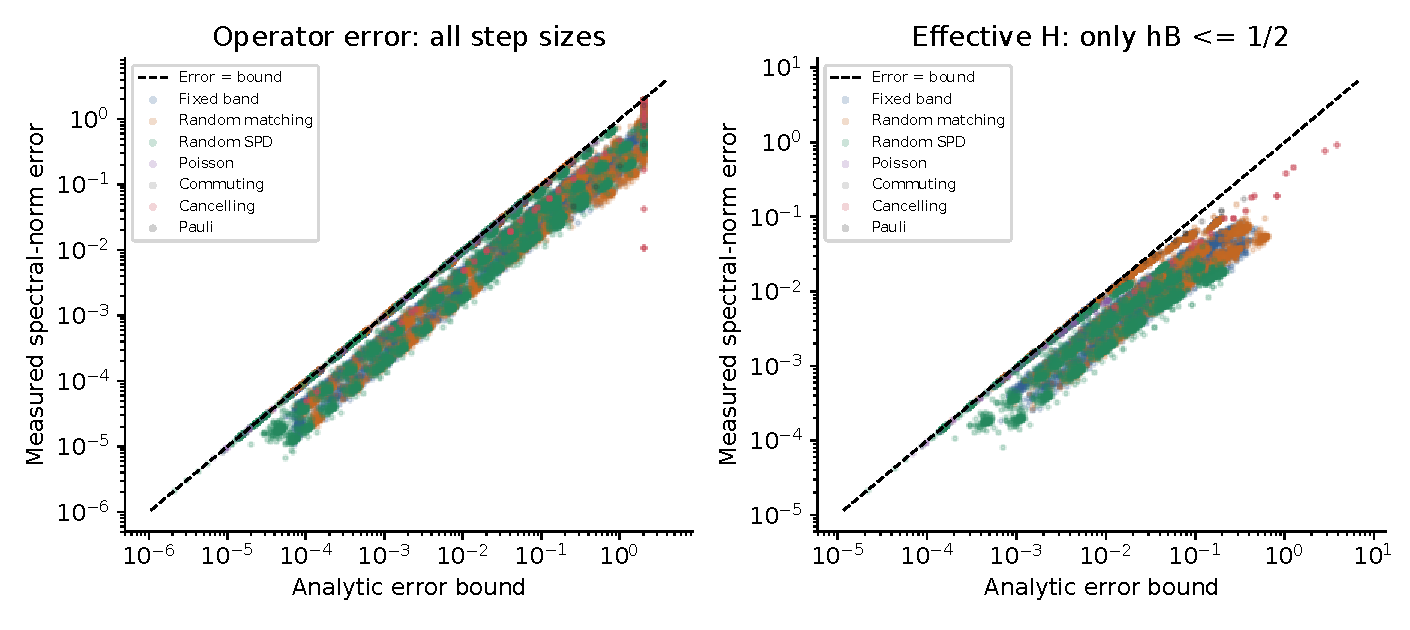
\includegraphics[width=\linewidth]{experiments/figures/actual_vs_bound.pdf}
\caption{Actual spectral-norm error versus its deterministic bound across the complete sweep. Each dot is a matrix/setting pair; the dashed diagonal denotes equality. Left: the operator bound includes the universal cap of 2. Right: only $hB\leq1/2$ is included, using the refined effective-H bound. Cases with $\CC=0$ are omitted from logarithmic comparisons and reported separately. Many points overlap.}
\end{figure}
\begin{figure}[p]
\centering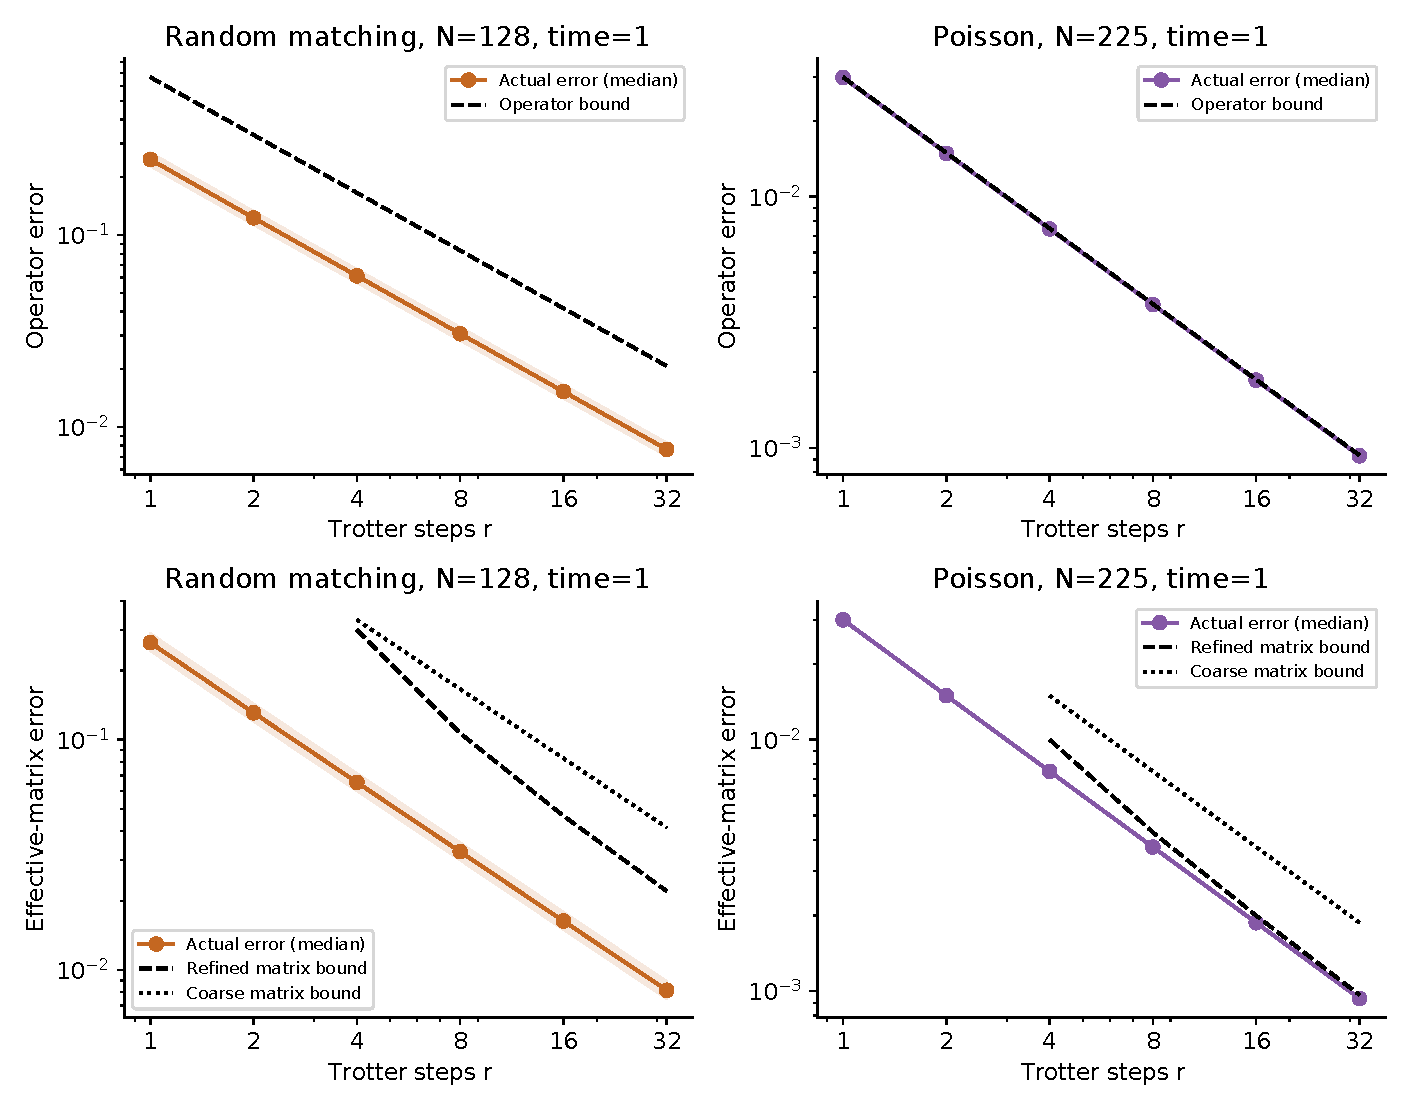
\includegraphics[width=\linewidth]{experiments/figures/step_convergence.pdf}
\caption{Increasing the number of steps at fixed $\tau=1$. Left: 16 random-matching matrices with $N=128$ and four matching terms; lines show medians, shaded areas the empirical 5th--95th percentiles. Right: the single $N=225$ Poisson matrix. Top: operator error and bound. Bottom: effective-H error, refined bound and coarse bound. Matrix bounds are drawn only when every sample at that point satisfies $hB\leq1/2$.}
\end{figure}
\clearpage
\begin{figure}[p]
\centering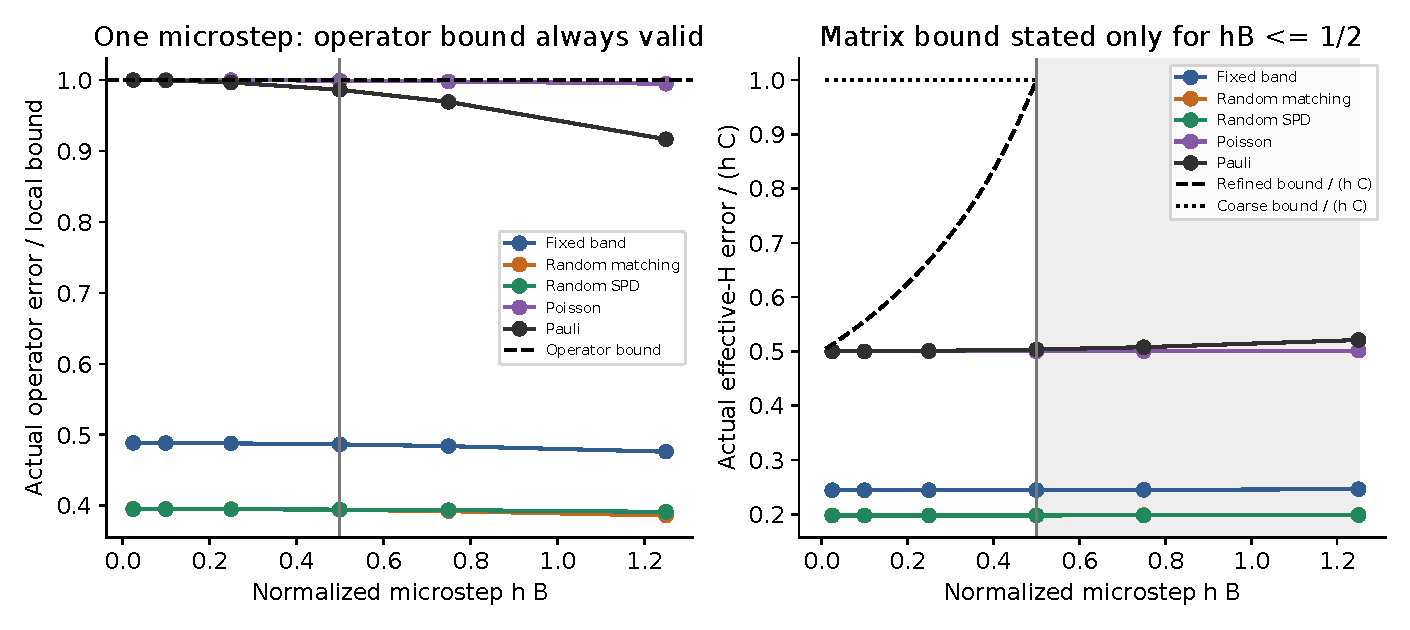
\includegraphics[width=\linewidth]{experiments/figures/branch_condition_sweep.pdf}
\caption{One-microstep experiments approaching and crossing $hB=1/2$. Synthetic curves use medians of the 16 samples with $N=128$ and four matching terms; Poisson uses $N=225$, and Pauli uses $N=2$. Left: actual operator error divided by $h^2\CC/2$, which is a bound at every step size. Right: actual effective-H error divided by $h\CC$. The refined bound becomes $1/[2(1-hB)]$ on the stated domain; the coarse bound becomes 1. The grey region is outside the sufficient condition, so it carries no claimed effective-H guarantee.}
\end{figure}
\begin{figure}[p]
\centering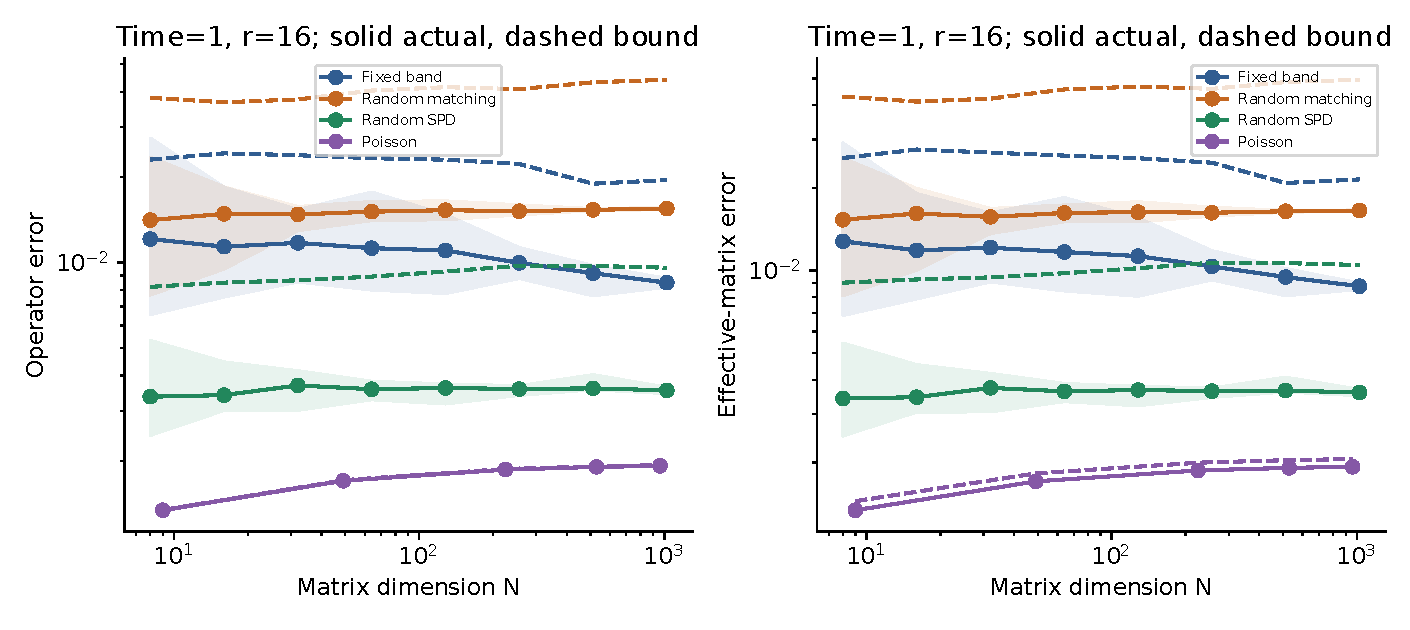
\includegraphics[width=\linewidth]{experiments/figures/dimension_sweep.pdf}
\caption{Dependence on dimension at fixed $\tau=1$, $r=16$, and four matching terms (plus the diagonal term for SPD/Poisson). Solid lines show median actual errors, dashed lines median bounds, and shading empirical 5th--95th percentiles. The Poisson family has one matrix at each dimension. Synthetic sample counts decrease with dimension as specified in the protocol; the two $N=1024$ samples are exploratory. This figure does not establish a universal asymptotic law in $N$.}
\end{figure}
\clearpage
\begin{figure}[ht]
\centering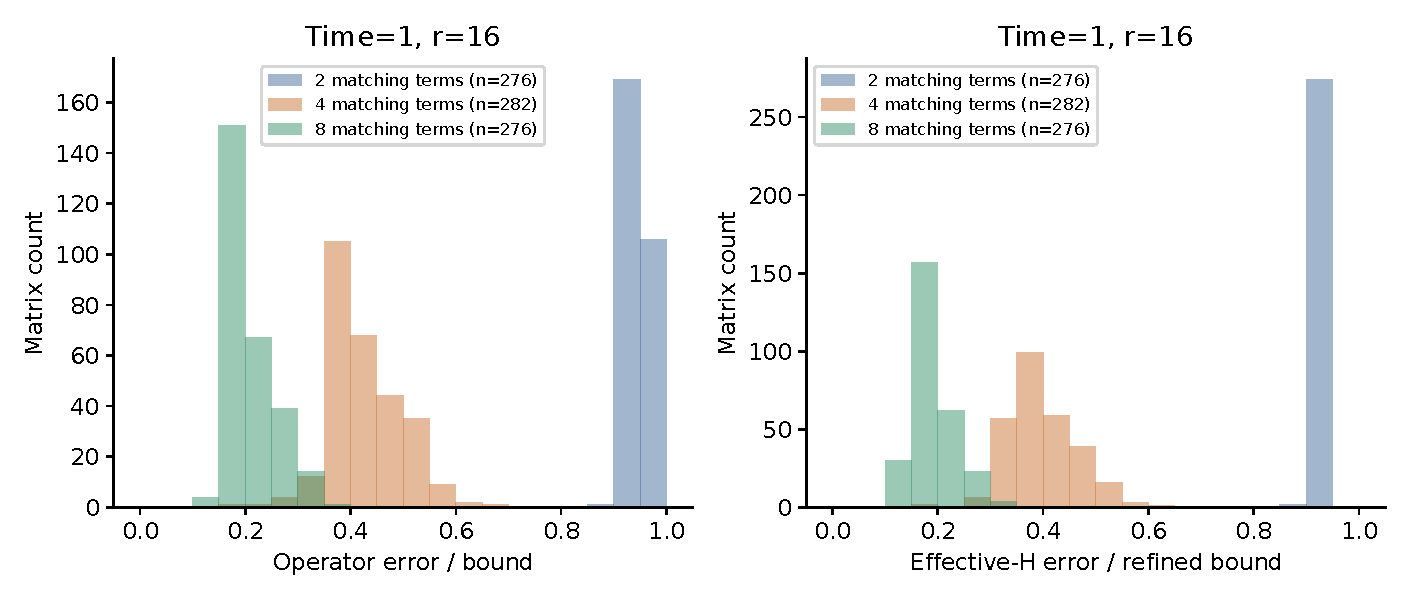
\includegraphics[width=\linewidth]{experiments/figures/ratio_distributions.pdf}
\caption{Error/bound ratios at a single setting ($\tau=1$, $r=16$), grouped by matching-term count and pooled over the three synthetic families and dimensions. Each matrix contributes once. Effective-H ratios include only the valid domain. These histograms describe the stated sampling design, not a universal distribution of sparse matrices.}
\end{figure}

\subsection{Branch wrapping is a different error}
For $H=\operatorname{diag}(1/2,1)$ with one commuting term, $P(h)^r=e^{\ii H\tau}$ exactly. Take $\tau=4$. For $r\geq8$, $hB\leq1/2$ and the microstep effective matrix equals $H$. However,
\begin{equation}
 \frac{\operatorname{Log}(P(h)^r)}{\ii\tau}
 =\operatorname{diag}(1/2,1-\pi/2),\qquad
 \left\lVert\frac{\operatorname{Log}(P(h)^r)}{\ii\tau}-H\right\rVert=\pi/2.
\end{equation}
Thus the global principal logarithm can retain a large discrepancy even when Trotter error vanishes. The accompanying diagonal diagnostic reproduces this example for $r=1,2,4,8,16,32,64,128$; it is separate from the 20,400 measurements above.

\subsection{Reproducibility and scope}
The folder \texttt{trotter-error/experiments/} contains the run script, Slurm submission, configurations, raw CSV data, grouped summaries, independent checks and PDF/PNG figures. Matrix seeds equal 20260909 plus the case ID. Pointwise 95\% bootstrap intervals for means in the summary CSV use 2,000 resamples of matrices (seed 20261909). Plot shading instead denotes empirical percentiles. Settings of the same matrix are correlated, so pooled ratio percentiles are descriptive and are not treated as independent samples. The deterministic proofs, rather than these experiments, establish validity for arbitrary finite dimensions. The observed coefficients depend on the family and decomposition; normalization alone does not fix them.
\clearpage

\begin{thebibliography}{1}
\bibitem{childs}
A.~M.~Childs, Y.~Su, M.~C.~Tran, N.~Wiebe, and S.~Zhu,
\emph{Theory of Trotter Error with Commutator Scaling},
Physical Review X \textbf{11}, 011020 (2021).
\href{https://doi.org/10.1103/PhysRevX.11.011020}{doi:10.1103/PhysRevX.11.011020}.
\href{https://arxiv.org/html/1912.08854v3}{arXiv:1912.08854v3}, Section 5.1, Proposition 15.
The pairwise first-order unitary estimate follows from that grouped-commutator bound. The logarithm-series and HHL perturbation arguments are derived explicitly in this note.
\end{thebibliography}
\end{document}
